%========================================================= HANDOUT OPTIONS =
% \documentclass[xcolor=dvipsnames,envcountsect,handout]{beamer}
%
% \mode<handout>
% % \mode<handout>{\beamertemplatesolidbackgroundcolor{black!2}}
% {
%  \usefonttheme{professionalfonts}
%  \setbeamertemplate{theorems}[numbered]
%  \setbeamertemplate{footline}{INF-UFG -- Tópicos Avançados de Programação \hfill\insertpagenumber\ --\ \insertpresentationendpage}
% }
%===========================================================================

%==================================================== PRESENTATION OPTIONS =
 \documentclass{beamer}

 \mode<presentation>
 {
   \usetheme[left]{Marburg}
   \usetheme{PaloAlto}

   \usefonttheme{serif}
 }

 \hypersetup{pdfpagemode=FullScreen}
%===========================================================================

%---------------------------------------------------------------- PACKAGES -
\usepackage[brazil]{babel}
\usepackage[T1]{fontenc}
\usepackage[ansinew]{inputenc}

%------------------------------------------------------------------- COVER -
\title[\bf Instituto\\ de\\ Informática\\ \large{UFG}]{{\bf\huge Maratona de Programação}}
\date{{\bf Instituto de Informática}\\ Universidade Federal de Goiás\\ \small{\url{ http://www.inf.ufg.br}}}
%\author[]{Cláudio Meneses {\Large\&} Humberto Longo}
\author[]{Humberto Longo}


\AtBeginSection[]
{
  \begin{frame}<beamer>
   \frametitle{}
   \begin{center}
    \begin{minipage}{.7\textwidth}
     \begin{block}{}
      \centering
      \huge
      \tt
      {\usebeamercolor[bg]{block title} \insertsection}
     \end{block}
    \end{minipage}
   \end{center}
  \end{frame}
}


%-------------------------------------------------------------------- FILES -
\includeonly
{
 TAP09-competicao,
 TAP09-olimpiada,
 TAP09-maratona,
 TAP09-preparacao,
 TAP09-topcoder,
 TAP09-tap,
}

%-------------------------------------------------------------------- TITLE -
\begin{document}

\begin{frame}
 \begin{block}{}
  \titlepage
 \end{block}
\end{frame}

%================================================================== SECTION -
\section{Introdução}
 \include{TAP09-competicao}

\section{Olimpíada}
 %- - - - - - - - - - - - - - - - - - - - - - - - - - - - - - - - - SLIDE -
\begin{frame}
 \frametitle{Competições de Programação}
 \begin{block}{\em International Olympiad in Informatics}
  \begin{overprint}
% .................................
   \onslide<1| handout:1>
   \begin{itemize}
    \item Idéia nasceu no congresso da UNESCO em 1987 na Bulgária. A primeira IOI ocorreu em 1989, também na Bulgária.
    \item O objetivo principal é estimular o interesse em Ciência da Computação, além de trazer talentos na área de todos os países do mundo que podem assim compartilhar experiências culturais e científicas.
    \item É uma das seis olimpíadas científicas reconhecidas.
    \item \url{http://en.wikipedia.org/wiki/International_Olympiad_in_Informatics}
   \end{itemize}
% .................................
   \onslide<2| handout:2>
   \begin{description}
    \item [2005] Novy Sacz, Polônia: \url{http://www.ioi2005.pl}
    \item [2006] Mérida, México: \url{http://www.ioi2006.org}
    \item [2007] Zagreb, Croácia: \url{http://ioi2007.hsin.hr}
    \item [2008] Cairo, Egito: \url{http://www.ioi2008.org}
    \item [2009] Plovdiv, Bulgária: \url{http://www.ioi2009.org}
    \item [2010] Waterloo, Ontario, Canada
    \item [2011] Tailândia
    \item [2012] Itália
   \end{description}
% .................................
  \end{overprint}
 \end{block}
\end{frame}
%- - - - - - - - - - - - - - - - - - - - - - - - - - - - - - - - - SLIDE -
\begin{frame}
 \frametitle{Competições de Programação}
 \begin{block}{Olimpíada Brasileira de Informática}
  \begin{itemize}
   \item OBI ocorre desde o ano de 1999.
   \item Evento da SBC desde seu início, coordenada pelo Prof. Ricardo Anido.
   \item Apoio do CNPq desde o ano de 2002.\medskip
   \item Para alunos de primeiro e segundo grau.
   \item Possui duas modalidades:
    \begin{itemize}
     \item Iniciação: para alunos até a oitava série do ensino fundamental.
     \item Programação: para alunos que cursam até o último ano do ensino médio.
    \end{itemize}
   \item Alunos que terminaram o segundo grau no ano anterior também podem participar da Olimpíada.
  \end{itemize}
 \end{block}
\end{frame}
%- - - - - - - - - - - - - - - - - - - - - - - - - - - - - - - - - SLIDE -
\begin{frame}
 \frametitle{Olimpíada de Informática}
 \begin{block}{Como funciona?}
  \begin{itemize}
   \item Na modalidade iniciação: provas de lógica em múltipla escolha para motivar o gosto pela ciência da computação.
   \item Você deve se inscrever em alguma instituição que vá aplicar a prova (escola ou
universidade).
   \item Na modalidade Programação você deve saber programar em C ou C++.
   \item A competição é individual.
   \item A competição é em três fases.
   \item As soluções são avaliadas a posteriori.
   \item Quanto mais testes um programa resolve (retorna o resultado esperado), maior a pontuação do competidor.
  \end{itemize}
 \end{block}
\end{frame}
%- - - - - - - - - - - - - - - - - - - - - - - - - - - - - - - - - SLIDE -
\begin{frame}
 \frametitle{Olimpíada de Informática}
 \begin{block}{E se eu me der bem?}
  \begin{itemize}
   \item Os melhores colocados são convidados a fazer um curso em Campinas.
   \item Dentre os participantes do curso serão escolhidos os integrantes da equipe
brasileira na Olimpíada Internacional de Informática (IOI).
  \end{itemize}
 \end{block}
\end{frame}
%- - - - - - - - - - - - - - - - - - - - - - - - - - - - - - - - - SLIDE -
% \begin{frame}
%  \frametitle{Olimpíada de Informática}
%  \begin{block}{Como Eu Me Preparo?}
%   \begin{itemize}
%    \item Os conceitos e as técnicas de programação serão estudados com base a linguagem de programação Objective CAML.
%     \begin{itemize}
%      \item Oportunamente, e para fins comparativos, poderão ser ilustrados alguns conceitos em uma segunda linguagem de programação, como C++.
%     \end{itemize}
%    \item O conteúdo da disciplina é incremental: os conceitos mais avançados apenas podem ser entendidos quando os conceitos básicos foram bem assimilados.
%    \item A disciplina DIM0424 fornecerá aos alunos oportunidade de exercitar de forma concreta os conceitos apresentados em sala de aula.
%    \item Atenção: o conteúdo da disciplina é abrangente e necessita um esforço importante e permanente dos alunos.
%    \item Os alunos recebem tarefas a serem realizadas antes da aula seguinte.
%   \end{itemize}
%  \end{block}
% \end{frame}
% %- - - - - - - - - - - - - - - - - - - - - - - - - - - - - - - - - SLIDE -


\section{Maratona}
 \include{TAP09-maratona}

\section{Preparação}
 \include{TAP09-preparacao}

\section{\em Top Coder}
 %- - - - - - - - - - - - - - - - - - - - - - - - - - - - - - - - - SLIDE -
\begin{frame}
 \frametitle{Competições de Programação}
 \begin{block}{\em Top Coder}
  \begin{itemize}
   \item Competição organizada por uma instituição não acadêmica com premiações em dinheiro.
   \item Para qualquer pessoa maior de 13 anos.
   \item Competições acontecem todas as semanas.
   \item Possui uma estrutura um pouco diferente das outras competições.
  \end{itemize}
 \end{block}
\end{frame}
%- - - - - - - - - - - - - - - - - - - - - - - - - - - - - - - - - SLIDE -
\begin{frame}
 \frametitle{\em Top Coder}
 \begin{block}{Como Funciona?}
  \begin{itemize}
   \item Você deve saber programar em C++, Java, C\# ou VB.
   \item A competição é individual.
   \item Objetivo é apresentar soluções corretas o mais rápido possível.
   \item Principiantes competem na segunda divisão.
   \item Participantes com uma pontuação acima de um determinado limiar passam a competir na primeira divisão.
  \end{itemize}
 \end{block}
\end{frame}
%- - - - - - - - - - - - - - - - - - - - - - - - - - - - - - - - - SLIDE -
\begin{frame}
 \frametitle{\em Top Coder}
 \begin{block}{E se eu me der bem?}
  \begin{itemize}
   \item Existe um ranking com os melhores competidores.
   \item Existem várias empresas patrocinando os eventos, querendo contratar bons profissionais.
   \item Algumas competições dão prêmios em dinheiro.
  \end{itemize}
 \end{block}
\end{frame}
%- - - - - - - - - - - - - - - - - - - - - - - - - - - - - - - - - SLIDE -
\begin{frame}
 \frametitle{\em Top Coder}
 \begin{block}{Como se Preparar?}
  \begin{itemize}
   \item Na página do TopCoder você pode praticar, resolvendo os problemas das competições passadas.
   \item \url{http://www.topcoder.com/tc}
  \end{itemize}
 \end{block}
\end{frame}
%- - - - - - - - - - - - - - - - - - - - - - - - - - - - - - - - - SLIDE -
\begin{frame}
 \frametitle{\em Top Coder}
 \begin{block}{Procedimento de registro}
  \centering
  \includegraphics[width=.9\textwidth]{figuras/topcoder}
 \end{block}
\end{frame}
%- - - - - - - - - - - - - - - - - - - - - - - - - - - - - - - - - SLIDE -
\begin{frame}
 \frametitle{\em Top Coder}
 \begin{block}{Procedimento de registro}
  \centering
  \includegraphics[width=.9\textwidth]{figuras/topcoder2}
 \end{block}
\end{frame}
%- - - - - - - - - - - - - - - - - - - - - - - - - - - - - - - - - SLIDE -


\section{TAP}
 %- - - - - - - - - - - - - - - - - - - - - - - - - - - - - - - - - SLIDE -
\begin{frame}
 \frametitle{Tópicos Avançados em Programação}
 \begin{block}{Metodologia}
  \begin{itemize}
   \item Apresentação de material em início da aula.
   \item Resolução de problema(s) durante o resto da aula.
   \item Resolução de problema(s) em trabalhos fora de aula (dever de casa).
   \item Divisão da disciplina:
    \begin{itemize}
     \item apresentação de recursos de linguagem.% [Vagner]
     \item apresentação de algumas (classes de) soluções clássicas.% [Humberto/Vagner]
     \item estudo e apresentação de soluções clássicas.% [Alunos]
    \end{itemize}
   \item O nível dos problemas deverá ir crescendo.
%    \item Modelo: \url{http://www.cs.sunysb.edu/~skiena/392/index.html}
  \end{itemize}
 \end{block}
\end{frame}
%- - - - - - - - - - - - - - - - - - - - - - - - - - - - - - - - - SLIDE -
\begin{frame}
 \frametitle{Tópicos Avançados em Programação}
 \begin{block}{Avaliação}
  \begin{itemize}
   \item Nota 1:
    \begin{description}[40\%]
     \item [30\%] Dever de casa.
     \item [30\%] Problemas resolvidos durante as aulas.
     \item [40\%] Desempenho durante a competição de avaliação.
    \end{description}
   \item Nota 2:
    \begin{description}[40\%]
     \item [30\%] Dever de casa.
     \item [30\%] Problemas resolvidos durante as aulas.
     \item [40\%] Desempenho durante a competição de avaliação.
    \end{description}
   \item Nota 3:
    \begin{description}[40\%]
     \item [30\%] Dever de casa.
     \item [30\%] Problemas resolvidos durante as aulas.
     \item [40\%] Desempenho durante a competição de avaliação.
    \end{description}
  \end{itemize}
 \end{block}
\end{frame}
%- - - - - - - - - - - - - - - - - - - - - - - - - - - - - - - - - SLIDE -
\begin{frame}
 \frametitle{Tópicos Avançados em Programação}
 \begin{block}{Avaliação}
  \begin{itemize}
   \item Pontos extras serão atribuídos às atividades extras.
   \item Prazos:
    \begin{itemize}
     \item O dever de casa deve ser entregue até a aula seguinte.
     \item Deveres de casa atrasados não serão aceitos.
    \end{itemize}
   \item Expectativa (dever de casa):
    \begin{itemize}
     \item Um problema por semana: nota entre 6 e 8.
     \item Dois problemas por semana: acima de 8.
    \end{itemize}
  \end{itemize}
 \end{block}
\end{frame}
%- - - - - - - - - - - - - - - - - - - - - - - - - - - - - - - - - SLIDE -
\begin{frame}
 \frametitle{Tópicos Avançados em Programação}
 \begin{block}{Bibliografia: livro texto}
  \centering
  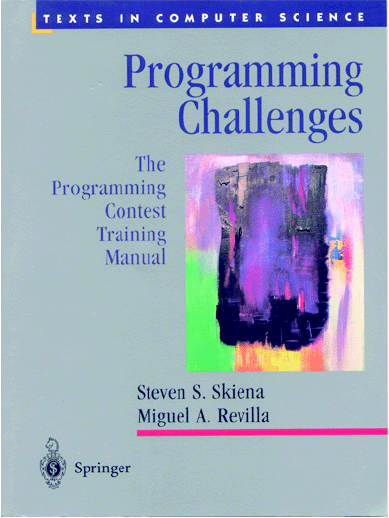
\includegraphics[height=.5\textheight]{figuras/prog-chall-book}
 \end{block}
 \begin{block}{}
  Art of Programming Contest. 2nd Edition. Ahmed Shamsul Arefin. ISBN 984-32-3382-4.
 \end{block}
\end{frame}
%- - - - - - - - - - - - - - - - - - - - - - - - - - - - - - - - - SLIDE -
\begin{frame}
 \frametitle{Tópicos Avançados em Programação}
 \begin{block}{Bibliografia: outros livros}
  \centering
  \includegraphics[width=.9\textwidth]{figuras/prog-books}
 \end{block}
\end{frame}
%- - - - - - - - - - - - - - - - - - - - - - - - - - - - - - - - - SLIDE -

%================================================================== SECTION -

\begin{frame}
 \begin{block}{}
  \titlepage
 \end{block}
\end{frame}
%- - - - - - - - - - - - - - - - - - - - - - - - - - - - - - - - - -  SLIDE -
\end{document}



